\documentclass[pdftex,12pt, oneside]{article}

%\usepackage[paperwidth=8.5in, paperheight=13in]{geometry} % Folio
\usepackage[paperwidth=8.27in, paperheight=11.69in]{geometry} % A4

\usepackage{makeidx}         % allows index generation
\usepackage{graphicx}        % standard LaTeX graphics tool
                             % when including figure files
\usepackage[bottom]{footmisc}% places footnotes at page bottom
\usepackage[english]{babel}
\usepackage{enumerate}
\usepackage{paralist}
\usepackage{float}
\usepackage{gensymb}  
\usepackage{listings}
\usepackage{color}
\usepackage{mathtools} % atau \usepackage{amsmath}
\renewcommand{\baselinestretch}{1.5}

\newcommand{\HRule}{\rule{\linewidth}{0.5mm}}

\definecolor{codegreen}{rgb}{0,0.6,0}
\definecolor{codegray}{rgb}{0.5,0.5,0.5}
\definecolor{codepurple}{rgb}{0.58,0,0.82}
\definecolor{backcolor}{rgb}{0.95,0.95,0.92}

\lstdefinestyle{mystyle}{
  backgroundcolor=\color{backcolor},
  commentstyle=\color{codegreen},
  keywordstyle=\color{magenta},
  stringstyle=\color{codepurple},
  basicstyle=\footnotesize,
  breakatwhitespace=false,
  breaklines=true,
  captionpos=b,
  keepspaces=true,
  numbers=left,
  numbersep=5pt,
  showspaces=false,
  showstringspaces=false,
  showtabs=false,
  tabsize=2
}

\lstset{style=mystyle}


\begin{document}
\sloppy % biar section ga melebar melewati kertas

\begin{center}
{\large PETUNJUK PEMAKAIAN DAN INSTALASI PROGRAM \textit{WEB SERVICES} PBB-P2}
\\[1cm]
25 November 2016\\
Priyanto Tamami, S.Kom.
\end{center}

%\frontmatter%%%%%%%%%%%%%%%%%%%%%%%%%%%%%%%%%%%%%%%%%%%%%%%%%%%%%%


%%%%%%%%%%%%%%%%%%%%%%%%%%%%%%%%%%%%%%%%%%%%%%%%%%%%%%%%%%%%%%%%%%%%%%

\section{INSTALASI PROGRAM}

Instalasi program aplikasi \textit{web services} ini cukup mudah, karena hasil dari kompilasi kode ke bentuk program akan berbentuk sebuah \textit{file} berekstensi \texttt{war}, yang nantinya \textit{file} ini akan diunggah pada \textit{server} Tomcat. Berikut adalah langkahnya :

\begin{enumerate}[1.]
  \item Melakukan kompilasi kode yang menghasilkan \textit{file} berekstensi \texttt{war}.
  \item Melakukan unggah \textit{file} \texttt{war} ke \textit{server} Tomcat seperti gambar \ref{fig:deploy-war} berikut :
  
  \begin{figure}[H]
    \centering
    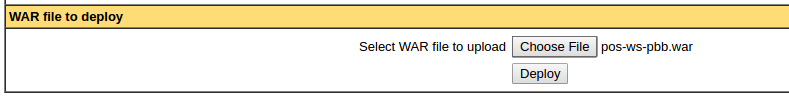
\includegraphics[width=1\textwidth]{./resources/001-deploy-war}
    \caption{\textit{Deploy file} \texttt{war}}
    \label{fig:deploy-war}
  \end{figure}
  
  \item Melakukan pengujian dengan melakukan akses ke \textit{server} menggunakan \textit{browser}, seperti terlihat pada gambar \ref{fig:ws-worked} :
  
  \begin{figure}[H]
    \centering
    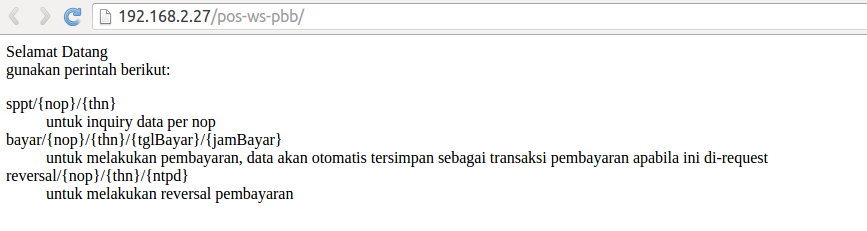
\includegraphics[width=0.8\textwidth]{./resources/002-ws-worked}
    \caption{Akses ke \textit{Web Services} Sudah Siap}
    \label{fig:ws-worked}
  \end{figure}
  
  \item Selesai.
\end{enumerate}


\section{PETUNJUK PEMAKAIAN}

Seperti terlihat pada halaman awal dari layanan \textit{web services}. Tiga layanan yang ditawarkan, yaitu \textit{inquiry} data, pencatatan pembayaran, dan \textit{reversal} pembayaran dapat dilakukan dengan perintah melalui URL \textit{web}.

Untuk mempermudah pemahaman, karena bentuknya hanya berupa \textit{web service} maka hanya akan 2 (dua) informasi yang dibutuhkan, yaitu berupa \textit{request} dan respon atau dalam kata lain \textit{input} dan \textit{output}. Berikut penjelasan lengkapnya :

\subsection{INPUT}

\subsubsection{\textit{INQUIRY} DATA TAGIHAN}

\textit{Request} yang pertama adalah untuk \textit{inquiry} data tagihan, format dari \textit{inquiry} data ini adalah sebagai berikut :

\begin{lstlisting}
/sppt/{nop}/{thn}
\end{lstlisting}

Dimana \texttt{nop} nantinya diganti dengan Nomor Objek Pajak (NOP) yang diinginkan dan \texttt{thn} digantikan dengan tahun pajak yang diinginkan.

\subsubsection{PENCATATAN PEMBAYARAN}

Untuk perintah yang kedua adalah \textit{request} untuk pencatatan pembayaran, perintahnya adalah sebagai berikut :

\begin{lstlisting}
/bayar/{nop}/{thn}/{tglBayar}/{jamBayar}
\end{lstlisting}

Untuk \texttt{nop} nantinya digantikan dengan Nomor Objek Pajak yang diinginkan, untuk \texttt{thn} digantikan dengan tahun pajak yang akan dibayarkan, untuk \texttt{tglBayar} digantikan dengan tanggal terjadinya pembayaran, dan untuk \texttt{jamBayar} digantikan dengan jam saat terjadinya pembayaran.

\subsubsection{\textit{REVERSAL} PEMBAYARAN}

Untuk perintah yang ketiga adalah \textit{request reversal} pembayaran bila terjadi kesalahan pembayaran. Format untuk perintah \textit{reversal} ini adalah sebagai berikut :

\begin{lstlisting}
/reversal/{nop}/{thn}/{ntpd}
\end{lstlisting}

Dimana \texttt{nop} digantikan dengan nomor objek pajak yang akan dilakukan \textit{reversal} pembayarannya, \texttt{thn} digantikan dengan tahun pajak yang diinginkan, dan \texttt{ntpd} digantikan dengan Nomor Transaksi Pajak Daerah yang dikirimkan melalui respon pada saat pencatatan pembayaran.


\subsection{OUTPUT} 

Bentuk keluaran yang dihasilkan sebagai \textit{respon} atas \textit{request} yang masuk secara garis besar pun dapat dibagi menjadi 3 (tiga) skenario, yaitu \textit{inquiry} data tagihan, pencatatan pembayaran, dan \textit{reversal} pembayaran. Secara detail dijelaskan sebagai berikut :

\subsubsection{\textit{INQUIRY} DATA TAGIHAN}

Respon atau keluaran dari \textit{server} untuk proses \textit{inquiry} data tagihan adalah sebagai berikut :

\begin{itemize}
  \item Skenario \textit{Inquiry} Yang Sukses
  
  Respon yang dihasilkan dari skenario ini adalah seperti berikut :
  
  \begin{lstlisting}
  {
    "code":01,
    "message":"Data ditemukan",
    "sppt": {
      "nop":"332901000100100010",
      "thn":"2013",
      "nama":{NAMA WP},
      "alamatOp":{KELURAHAN - KECAMATAN},
      "pokok":35750,
      "denda":0
    }
  }
  \end{lstlisting}
  
  \texttt{\{NAMA WP\}} ini nantinya berisi nama wajib pajak yang tertera pada SPPT, dan \texttt{\{KELURAHAN - KECAMATAN\}} berisi alamat objek pajak berupa Kelurahan dan Kecamatan dimana objek pajak tersebut berada.
  
  \item Skenario \textit{Inquiry} Yang Gagal Karena Tahun Pajak Bukan Angka
  
  Respon yang dihasilkan dari skenario ini adalah sebagai berikut :
  
  \begin{lstlisting}
  {
    "code":36,
    "message":"Tahun Pajak Mengandung Karakter bukan Angka",
    "sppt":null
  }
  \end{lstlisting}
  
  \item Skenario \textit{Inquiry} Yang Gagal Karena Data Tidak Ditemukan
  
  Respon yang dihasilkan untuk skenario ini adalah sebagai berikut :
  
  \begin{lstlisting}
  {
    "code":10,
    "message":"Data Tidak Ditemukan",
    "sppt":null
  }
  \end{lstlisting}
  
  \item Skenario \textit{Inquiry} Yang Gagal Karena Kesalahan \textit{Server}
  
  Respon yang dihasilkan untuk skenario ini adalah sebagai berikut :
  
  \begin{lstlisting}
  {
    "code":04,
    "message":"Kesalahan DB",
    "sppt":null
  }
  \end{lstlisting}
  
\end{itemize}

\subsubsection{PENCATATAN PEMBAYARAN}

Respon dari \textit{server} untuk proses pencatatan pembayaran adalah sebagai berikut :

\begin{itemize}
  \item Skenario Pencatatan Pembayaran Yang Sukses
  
  Respon yang dihasilkan untuk skenario ini adalah sebagai berikut :
  
  \begin{lstlisting}
  {
    "code":01,
    "message":"Pembayaran Telah Tercatat",
    "byrSppt":{
      "nop":{NOP},
      "thn":{THN},
      "ntpd":{NTPD},
      "mataAnggaranPokok":"4.1.1.11.02",
      "pokok":9350,
      "mataAnggaranSanksi":"4.1.1.11.02",
      "sanksi":0,
      "namaWp":{NAMA WP},
      "alamatOp":{KELURAHAN - KECAMATAN}
    }
  }
  \end{lstlisting}
  
  Penjelasan dari kode diatas adalah seperti ini, \texttt{\{NOP\}} nantinya akan berisi nomor objek pajak yang di-\textit{request} untuk dicatatkan pembayarannya, \texttt{\{THN\}} nantinya berisi tahun pajak yang dicatatkan pembayarannya, \texttt{\{NTPD\}} nantinya berisi nomor transaksi pajak daerah sebagai tanda bahwa \textit{request} pencatatan pembayaran telah berhasil diproses, \texttt{\{NAMA WP\}} akan berisi nama wajib pajak yang dicatatkan pembayarannya, dan \texttt{\{KELURAHAN - KECAMATAN\}} akan berisi nama Kelurahan/Desa dan Kecamatan tempat objek pajak berada.
  
  \item Skenario Pencatatan Pembayaran Yang Gagal Karena Jam Pembayaran Melebihi Jam Pencatatan
  
  Respon dari hasil \textit{request} untuk skenario ini adalah sebagai berikut :
  
  \begin{lstlisting}
  {
    "code":32,
    "message":"Tanggal atau jam pada saat dibayarkan melebihi tanggal dan jam saat ini",
    "byrSppt":null
  }
  \end{lstlisting}
  
  \item Skenario Pencatatan Pembayaran Yang Gagal Karena Tagihan Telah Terbayar Atau Nihil
  
  Respon dari hasil \textit{request} untuk skenario ini adalah sebagai berikut :
  
  \begin{lstlisting}
  {
    "code":13,
    "message":"Tagihan Telah Terbayar",
    "byrSppt":null
  }
  \end{lstlisting}
  
  \item Skenario Pencatatan Pembayaran Yang Gagal Karena Telah Dibatalkan
  
  Respon dari hasil \textit{request} untuk skenario ini adalah sebagai berikut :
  
  \begin{lstlisting}
  {
    "code":03,
    "message":"Tagihan SPPT Telah Dibatalkan",
    "byrSppt":null
  }
  \end{lstlisting}
  
  \item Skenario Pencatatan Pembayaran Yang Gagal Karena Kesalahan \textit{Server}
  
  Respon dari hasil \textit{request} untuk skenario ini adalah sebagai berikut :
  
  \begin{lstlisting}
  {
    "code":04,
    "message":"Kesalahan Server",
    "byrSppt":null
  }
  \end{lstlisting}
  
\end{itemize}

\subsubsection{\textit{REVERSAL} PEMBAYARAN}

Respon dari \textit{server} untuk proses \textit{reversal} pembayaran adalah sebagai berikut :

\begin{itemize}
  \item Skenario \textit{Reversal} Pembayaran Yang Sukses
  
  Respon dari \textit{request} untuk skenario ini adalah sebagai berikut :
  
  \begin{lstlisting}
  {
    "code":01,
    "message":"Proses Reversal Berhasil",
    "revPembayaran":{
      "nop":{NOP},
      "thn":{THN},
      "ntpd":{NTPD}
    }
  }
  \end{lstlisting}
  
  Keterangannya adalah sebagai berikut, \texttt{\{NOP\}} nantinya akan berisi nomor objek pajak yang akan dilakukan \textit{reversal} pembayarannya, \texttt{\{THN\}} akan berisi tahun pajak yang akan dilakukan proses \textit{reversal} terhadap pembayarannya, dan \texttt{\{NTPD\}} adalah nomor transaksi pajak daerah yang dikirimkan pada saat transaksi pencatatan pembayaran.
  
  \item Skenario \textit{Reversal} Pembayaran Yang Gagal Karena Data Yang Diminta Tidak Ada
  
  Respon dari \textit{request} untuk skenario ini adalah sebagai berikut :
  
  \begin{lstlisting}
  {
    "code":01,
    "message":"Data Yang Diminta Tidak Ada",
    "revPembayaran":null
    }
  }
  \end{lstlisting}
  
  \item Skenario \textit{Reversal} Pembayaran Yang Gagal Karena Ada Data Pembayaran Yang Tercatat Ganda
  
  Respon dari \textit{request} untuk skenario ini adalah sebagai berikut :
  
  \begin{lstlisting}
  {
    "code":04,
    "message":"Data tersebut Ganda",
    "revPembayaran":null
  }
  \end{lstlisting}
  
  \item Skenario \textit{Reversal} Pembayaran Yang Gagal Karena Kesalahan Server
  
  Respon dari \textit{request} untuk skenario ini adalah sebagai berikut :
  
  \begin{lstlisting}
  {
    "code":04,
    "message":"Kesalahan Server",
    "revPembayaran":null
  }
  \end{lstlisting}
  
\end{itemize}

\end{document}